% Created by tikzDevice version 0.7.0 on 2014-06-17 19:19:06
% !TEX encoding = UTF-8 Unicode
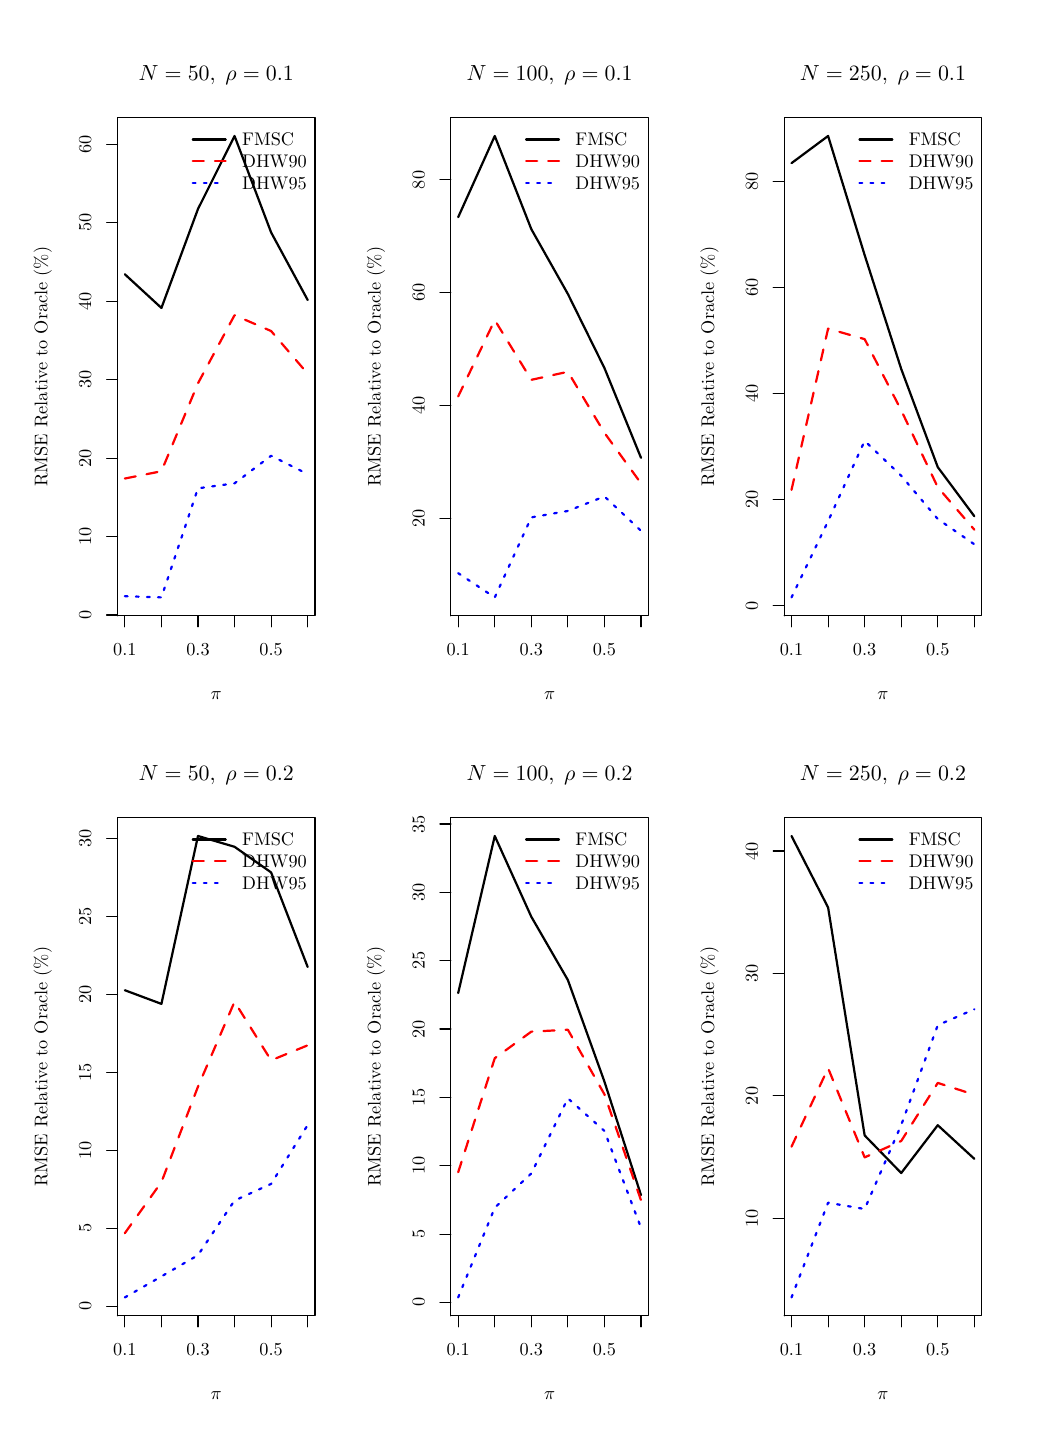
\begin{tikzpicture}[x=1pt,y=1pt]
\definecolor[named]{fillColor}{rgb}{1.00,1.00,1.00}
\path[use as bounding box,fill=fillColor,fill opacity=0.00] (0,0) rectangle (361.35,505.89);
\begin{scope}
\path[clip] ( 32.47,293.34) rectangle (103.82,473.42);
\definecolor[named]{drawColor}{rgb}{0.00,0.00,0.00}

\path[draw=drawColor,line width= 0.8pt,line join=round,line cap=round] ( 35.11,416.78) --
	( 48.33,404.60) --
	( 61.54,440.36) --
	( 74.75,466.75) --
	( 87.96,431.91) --
	(101.18,407.48);
\end{scope}
\begin{scope}
\path[clip] (  0.00,  0.00) rectangle (361.35,505.89);
\definecolor[named]{drawColor}{rgb}{0.00,0.00,0.00}

\path[draw=drawColor,line width= 0.4pt,line join=round,line cap=round] ( 35.11,293.34) -- (101.18,293.34);

\path[draw=drawColor,line width= 0.4pt,line join=round,line cap=round] ( 35.11,293.34) -- ( 35.11,289.38);

\path[draw=drawColor,line width= 0.4pt,line join=round,line cap=round] ( 48.33,293.34) -- ( 48.33,289.38);

\path[draw=drawColor,line width= 0.4pt,line join=round,line cap=round] ( 61.54,293.34) -- ( 61.54,289.38);

\path[draw=drawColor,line width= 0.4pt,line join=round,line cap=round] ( 74.75,293.34) -- ( 74.75,289.38);

\path[draw=drawColor,line width= 0.4pt,line join=round,line cap=round] ( 87.96,293.34) -- ( 87.96,289.38);

\path[draw=drawColor,line width= 0.4pt,line join=round,line cap=round] (101.18,293.34) -- (101.18,289.38);

\node[text=drawColor,anchor=base,inner sep=0pt, outer sep=0pt, scale=  0.66] at ( 35.11,279.08) {0.1};

\node[text=drawColor,anchor=base,inner sep=0pt, outer sep=0pt, scale=  0.66] at ( 61.54,279.08) {0.3};

\node[text=drawColor,anchor=base,inner sep=0pt, outer sep=0pt, scale=  0.66] at ( 87.96,279.08) {0.5};

\path[draw=drawColor,line width= 0.4pt,line join=round,line cap=round] ( 32.47,293.67) -- ( 32.47,463.71);

\path[draw=drawColor,line width= 0.4pt,line join=round,line cap=round] ( 32.47,293.67) -- ( 28.51,293.67);

\path[draw=drawColor,line width= 0.4pt,line join=round,line cap=round] ( 32.47,322.01) -- ( 28.51,322.01);

\path[draw=drawColor,line width= 0.4pt,line join=round,line cap=round] ( 32.47,350.35) -- ( 28.51,350.35);

\path[draw=drawColor,line width= 0.4pt,line join=round,line cap=round] ( 32.47,378.69) -- ( 28.51,378.69);

\path[draw=drawColor,line width= 0.4pt,line join=round,line cap=round] ( 32.47,407.03) -- ( 28.51,407.03);

\path[draw=drawColor,line width= 0.4pt,line join=round,line cap=round] ( 32.47,435.37) -- ( 28.51,435.37);

\path[draw=drawColor,line width= 0.4pt,line join=round,line cap=round] ( 32.47,463.71) -- ( 28.51,463.71);

\node[text=drawColor,rotate= 90.00,anchor=base,inner sep=0pt, outer sep=0pt, scale=  0.66] at ( 22.97,293.67) {0};

\node[text=drawColor,rotate= 90.00,anchor=base,inner sep=0pt, outer sep=0pt, scale=  0.66] at ( 22.97,322.01) {10};

\node[text=drawColor,rotate= 90.00,anchor=base,inner sep=0pt, outer sep=0pt, scale=  0.66] at ( 22.97,350.35) {20};

\node[text=drawColor,rotate= 90.00,anchor=base,inner sep=0pt, outer sep=0pt, scale=  0.66] at ( 22.97,378.69) {30};

\node[text=drawColor,rotate= 90.00,anchor=base,inner sep=0pt, outer sep=0pt, scale=  0.66] at ( 22.97,407.03) {40};

\node[text=drawColor,rotate= 90.00,anchor=base,inner sep=0pt, outer sep=0pt, scale=  0.66] at ( 22.97,435.37) {50};

\node[text=drawColor,rotate= 90.00,anchor=base,inner sep=0pt, outer sep=0pt, scale=  0.66] at ( 22.97,463.71) {60};

\path[draw=drawColor,line width= 0.4pt,line join=round,line cap=round] ( 32.47,293.34) --
	(103.82,293.34) --
	(103.82,473.42) --
	( 32.47,473.42) --
	( 32.47,293.34);
\end{scope}
\begin{scope}
\path[clip] (  0.00,252.94) rectangle (120.45,505.89);
\definecolor[named]{drawColor}{rgb}{0.00,0.00,0.00}

\node[text=drawColor,anchor=base,inner sep=0pt, outer sep=0pt, scale=  0.79] at ( 68.14,486.92) {\bfseries $N=50, \;\rho=0.1$};

\node[text=drawColor,anchor=base,inner sep=0pt, outer sep=0pt, scale=  0.66] at ( 68.14,263.24) {$\pi$};

\node[text=drawColor,rotate= 90.00,anchor=base,inner sep=0pt, outer sep=0pt, scale=  0.66] at (  7.13,383.38) {RMSE Relative to Oracle (\%)};
\end{scope}
\begin{scope}
\path[clip] ( 32.47,293.34) rectangle (103.82,473.42);
\definecolor[named]{drawColor}{rgb}{1.00,0.00,0.00}

\path[draw=drawColor,line width= 0.8pt,dash pattern=on 4pt off 4pt ,line join=round,line cap=round] ( 35.11,342.97) --
	( 48.33,345.60) --
	( 61.54,377.38) --
	( 74.75,401.99) --
	( 87.96,396.27) --
	(101.18,380.84);
\definecolor[named]{drawColor}{rgb}{0.00,0.00,1.00}

\path[draw=drawColor,line width= 0.8pt,dash pattern=on 1pt off 3pt ,line join=round,line cap=round] ( 35.11,300.45) --
	( 48.33,300.01) --
	( 61.54,339.43) --
	( 74.75,341.23) --
	( 87.96,351.19) --
	(101.18,344.57);
\definecolor[named]{drawColor}{rgb}{0.00,0.00,0.00}

\path[draw=drawColor,line width= 0.8pt,line join=round,line cap=round] ( 59.66,465.50) -- ( 71.54,465.50);
\definecolor[named]{drawColor}{rgb}{1.00,0.00,0.00}

\path[draw=drawColor,line width= 0.8pt,dash pattern=on 4pt off 4pt ,line join=round,line cap=round] ( 59.66,457.58) -- ( 71.54,457.58);
\definecolor[named]{drawColor}{rgb}{0.00,0.00,1.00}

\path[draw=drawColor,line width= 0.8pt,dash pattern=on 1pt off 3pt ,line join=round,line cap=round] ( 59.66,449.66) -- ( 71.54,449.66);
\definecolor[named]{drawColor}{rgb}{0.00,0.00,0.00}

\node[text=drawColor,anchor=base west,inner sep=0pt, outer sep=0pt, scale=  0.66] at ( 77.48,463.23) {FMSC};

\node[text=drawColor,anchor=base west,inner sep=0pt, outer sep=0pt, scale=  0.66] at ( 77.48,455.31) {DHW90};

\node[text=drawColor,anchor=base west,inner sep=0pt, outer sep=0pt, scale=  0.66] at ( 77.48,447.39) {DHW95};
\end{scope}
\begin{scope}
\path[clip] ( 32.47, 40.39) rectangle (103.82,220.47);
\definecolor[named]{drawColor}{rgb}{0.00,0.00,0.00}

\path[draw=drawColor,line width= 0.8pt,line join=round,line cap=round] ( 35.11,158.07) --
	( 48.33,153.13) --
	( 61.54,213.80) --
	( 74.75,209.90) --
	( 87.96,200.65) --
	(101.18,166.47);
\end{scope}
\begin{scope}
\path[clip] (  0.00,  0.00) rectangle (361.35,505.89);
\definecolor[named]{drawColor}{rgb}{0.00,0.00,0.00}

\path[draw=drawColor,line width= 0.4pt,line join=round,line cap=round] ( 35.11, 40.39) -- (101.18, 40.39);

\path[draw=drawColor,line width= 0.4pt,line join=round,line cap=round] ( 35.11, 40.39) -- ( 35.11, 36.43);

\path[draw=drawColor,line width= 0.4pt,line join=round,line cap=round] ( 48.33, 40.39) -- ( 48.33, 36.43);

\path[draw=drawColor,line width= 0.4pt,line join=round,line cap=round] ( 61.54, 40.39) -- ( 61.54, 36.43);

\path[draw=drawColor,line width= 0.4pt,line join=round,line cap=round] ( 74.75, 40.39) -- ( 74.75, 36.43);

\path[draw=drawColor,line width= 0.4pt,line join=round,line cap=round] ( 87.96, 40.39) -- ( 87.96, 36.43);

\path[draw=drawColor,line width= 0.4pt,line join=round,line cap=round] (101.18, 40.39) -- (101.18, 36.43);

\node[text=drawColor,anchor=base,inner sep=0pt, outer sep=0pt, scale=  0.66] at ( 35.11, 26.14) {0.1};

\node[text=drawColor,anchor=base,inner sep=0pt, outer sep=0pt, scale=  0.66] at ( 61.54, 26.14) {0.3};

\node[text=drawColor,anchor=base,inner sep=0pt, outer sep=0pt, scale=  0.66] at ( 87.96, 26.14) {0.5};

\path[draw=drawColor,line width= 0.4pt,line join=round,line cap=round] ( 32.47, 43.89) -- ( 32.47,213.00);

\path[draw=drawColor,line width= 0.4pt,line join=round,line cap=round] ( 32.47, 43.89) -- ( 28.51, 43.89);

\path[draw=drawColor,line width= 0.4pt,line join=round,line cap=round] ( 32.47, 72.07) -- ( 28.51, 72.07);

\path[draw=drawColor,line width= 0.4pt,line join=round,line cap=round] ( 32.47,100.26) -- ( 28.51,100.26);

\path[draw=drawColor,line width= 0.4pt,line join=round,line cap=round] ( 32.47,128.44) -- ( 28.51,128.44);

\path[draw=drawColor,line width= 0.4pt,line join=round,line cap=round] ( 32.47,156.63) -- ( 28.51,156.63);

\path[draw=drawColor,line width= 0.4pt,line join=round,line cap=round] ( 32.47,184.81) -- ( 28.51,184.81);

\path[draw=drawColor,line width= 0.4pt,line join=round,line cap=round] ( 32.47,213.00) -- ( 28.51,213.00);

\node[text=drawColor,rotate= 90.00,anchor=base,inner sep=0pt, outer sep=0pt, scale=  0.66] at ( 22.97, 43.89) {0};

\node[text=drawColor,rotate= 90.00,anchor=base,inner sep=0pt, outer sep=0pt, scale=  0.66] at ( 22.97, 72.07) {5};

\node[text=drawColor,rotate= 90.00,anchor=base,inner sep=0pt, outer sep=0pt, scale=  0.66] at ( 22.97,100.26) {10};

\node[text=drawColor,rotate= 90.00,anchor=base,inner sep=0pt, outer sep=0pt, scale=  0.66] at ( 22.97,128.44) {15};

\node[text=drawColor,rotate= 90.00,anchor=base,inner sep=0pt, outer sep=0pt, scale=  0.66] at ( 22.97,156.63) {20};

\node[text=drawColor,rotate= 90.00,anchor=base,inner sep=0pt, outer sep=0pt, scale=  0.66] at ( 22.97,184.81) {25};

\node[text=drawColor,rotate= 90.00,anchor=base,inner sep=0pt, outer sep=0pt, scale=  0.66] at ( 22.97,213.00) {30};

\path[draw=drawColor,line width= 0.4pt,line join=round,line cap=round] ( 32.47, 40.39) --
	(103.82, 40.39) --
	(103.82,220.47) --
	( 32.47,220.47) --
	( 32.47, 40.39);
\end{scope}
\begin{scope}
\path[clip] (  0.00,  0.00) rectangle (120.45,252.94);
\definecolor[named]{drawColor}{rgb}{0.00,0.00,0.00}

\node[text=drawColor,anchor=base,inner sep=0pt, outer sep=0pt, scale=  0.79] at ( 68.14,233.98) {\bfseries $N=50, \;\rho=0.2$};

\node[text=drawColor,anchor=base,inner sep=0pt, outer sep=0pt, scale=  0.66] at ( 68.14, 10.30) {$\pi$};

\node[text=drawColor,rotate= 90.00,anchor=base,inner sep=0pt, outer sep=0pt, scale=  0.66] at (  7.13,130.43) {RMSE Relative to Oracle (\%)};
\end{scope}
\begin{scope}
\path[clip] ( 32.47, 40.39) rectangle (103.82,220.47);
\definecolor[named]{drawColor}{rgb}{1.00,0.00,0.00}

\path[draw=drawColor,line width= 0.8pt,dash pattern=on 4pt off 4pt ,line join=round,line cap=round] ( 35.11, 70.27) --
	( 48.33, 88.73) --
	( 61.54,123.22) --
	( 74.75,153.91) --
	( 87.96,132.73) --
	(101.18,138.16);
\definecolor[named]{drawColor}{rgb}{0.00,0.00,1.00}

\path[draw=drawColor,line width= 0.8pt,dash pattern=on 1pt off 3pt ,line join=round,line cap=round] ( 35.11, 47.06) --
	( 48.33, 54.66) --
	( 61.54, 62.33) --
	( 74.75, 82.07) --
	( 87.96, 88.09) --
	(101.18,109.36);
\definecolor[named]{drawColor}{rgb}{0.00,0.00,0.00}

\path[draw=drawColor,line width= 0.8pt,line join=round,line cap=round] ( 59.66,212.55) -- ( 71.54,212.55);
\definecolor[named]{drawColor}{rgb}{1.00,0.00,0.00}

\path[draw=drawColor,line width= 0.8pt,dash pattern=on 4pt off 4pt ,line join=round,line cap=round] ( 59.66,204.63) -- ( 71.54,204.63);
\definecolor[named]{drawColor}{rgb}{0.00,0.00,1.00}

\path[draw=drawColor,line width= 0.8pt,dash pattern=on 1pt off 3pt ,line join=round,line cap=round] ( 59.66,196.71) -- ( 71.54,196.71);
\definecolor[named]{drawColor}{rgb}{0.00,0.00,0.00}

\node[text=drawColor,anchor=base west,inner sep=0pt, outer sep=0pt, scale=  0.66] at ( 77.48,210.28) {FMSC};

\node[text=drawColor,anchor=base west,inner sep=0pt, outer sep=0pt, scale=  0.66] at ( 77.48,202.36) {DHW90};

\node[text=drawColor,anchor=base west,inner sep=0pt, outer sep=0pt, scale=  0.66] at ( 77.48,194.44) {DHW95};
\end{scope}
\begin{scope}
\path[clip] (152.92,293.34) rectangle (224.27,473.42);
\definecolor[named]{drawColor}{rgb}{0.00,0.00,0.00}

\path[draw=drawColor,line width= 0.8pt,line join=round,line cap=round] (155.56,437.40) --
	(168.78,466.75) --
	(181.99,433.08) --
	(195.20,409.66) --
	(208.41,382.90) --
	(221.63,350.44);
\end{scope}
\begin{scope}
\path[clip] (  0.00,  0.00) rectangle (361.35,505.89);
\definecolor[named]{drawColor}{rgb}{0.00,0.00,0.00}

\path[draw=drawColor,line width= 0.4pt,line join=round,line cap=round] (155.56,293.34) -- (221.63,293.34);

\path[draw=drawColor,line width= 0.4pt,line join=round,line cap=round] (155.56,293.34) -- (155.56,289.38);

\path[draw=drawColor,line width= 0.4pt,line join=round,line cap=round] (168.78,293.34) -- (168.78,289.38);

\path[draw=drawColor,line width= 0.4pt,line join=round,line cap=round] (181.99,293.34) -- (181.99,289.38);

\path[draw=drawColor,line width= 0.4pt,line join=round,line cap=round] (195.20,293.34) -- (195.20,289.38);

\path[draw=drawColor,line width= 0.4pt,line join=round,line cap=round] (208.41,293.34) -- (208.41,289.38);

\path[draw=drawColor,line width= 0.4pt,line join=round,line cap=round] (221.63,293.34) -- (221.63,289.38);

\node[text=drawColor,anchor=base,inner sep=0pt, outer sep=0pt, scale=  0.66] at (155.56,279.08) {0.1};

\node[text=drawColor,anchor=base,inner sep=0pt, outer sep=0pt, scale=  0.66] at (181.99,279.08) {0.3};

\node[text=drawColor,anchor=base,inner sep=0pt, outer sep=0pt, scale=  0.66] at (208.41,279.08) {0.5};

\path[draw=drawColor,line width= 0.4pt,line join=round,line cap=round] (152.92,328.65) -- (152.92,450.88);

\path[draw=drawColor,line width= 0.4pt,line join=round,line cap=round] (152.92,328.65) -- (148.96,328.65);

\path[draw=drawColor,line width= 0.4pt,line join=round,line cap=round] (152.92,369.39) -- (148.96,369.39);

\path[draw=drawColor,line width= 0.4pt,line join=round,line cap=round] (152.92,410.14) -- (148.96,410.14);

\path[draw=drawColor,line width= 0.4pt,line join=round,line cap=round] (152.92,450.88) -- (148.96,450.88);

\node[text=drawColor,rotate= 90.00,anchor=base,inner sep=0pt, outer sep=0pt, scale=  0.66] at (143.42,328.65) {20};

\node[text=drawColor,rotate= 90.00,anchor=base,inner sep=0pt, outer sep=0pt, scale=  0.66] at (143.42,369.39) {40};

\node[text=drawColor,rotate= 90.00,anchor=base,inner sep=0pt, outer sep=0pt, scale=  0.66] at (143.42,410.14) {60};

\node[text=drawColor,rotate= 90.00,anchor=base,inner sep=0pt, outer sep=0pt, scale=  0.66] at (143.42,450.88) {80};

\path[draw=drawColor,line width= 0.4pt,line join=round,line cap=round] (152.92,293.34) --
	(224.27,293.34) --
	(224.27,473.42) --
	(152.92,473.42) --
	(152.92,293.34);
\end{scope}
\begin{scope}
\path[clip] (120.45,252.94) rectangle (240.90,505.89);
\definecolor[named]{drawColor}{rgb}{0.00,0.00,0.00}

\node[text=drawColor,anchor=base,inner sep=0pt, outer sep=0pt, scale=  0.79] at (188.59,486.92) {\bfseries $N=100, \;\rho=0.1$};

\node[text=drawColor,anchor=base,inner sep=0pt, outer sep=0pt, scale=  0.66] at (188.59,263.24) {$\pi$};

\node[text=drawColor,rotate= 90.00,anchor=base,inner sep=0pt, outer sep=0pt, scale=  0.66] at (127.58,383.38) {RMSE Relative to Oracle (\%)};
\end{scope}
\begin{scope}
\path[clip] (152.92,293.34) rectangle (224.27,473.42);
\definecolor[named]{drawColor}{rgb}{1.00,0.00,0.00}

\path[draw=drawColor,line width= 0.8pt,dash pattern=on 4pt off 4pt ,line join=round,line cap=round] (155.56,372.63) --
	(168.78,400.22) --
	(181.99,378.63) --
	(195.20,381.55) --
	(208.41,359.49) --
	(221.63,341.22);
\definecolor[named]{drawColor}{rgb}{0.00,0.00,1.00}

\path[draw=drawColor,line width= 0.8pt,dash pattern=on 1pt off 3pt ,line join=round,line cap=round] (155.56,308.77) --
	(168.78,300.01) --
	(181.99,328.93) --
	(195.20,331.26) --
	(208.41,336.50) --
	(221.63,324.08);
\definecolor[named]{drawColor}{rgb}{0.00,0.00,0.00}

\path[draw=drawColor,line width= 0.8pt,line join=round,line cap=round] (180.11,465.50) -- (191.99,465.50);
\definecolor[named]{drawColor}{rgb}{1.00,0.00,0.00}

\path[draw=drawColor,line width= 0.8pt,dash pattern=on 4pt off 4pt ,line join=round,line cap=round] (180.11,457.58) -- (191.99,457.58);
\definecolor[named]{drawColor}{rgb}{0.00,0.00,1.00}

\path[draw=drawColor,line width= 0.8pt,dash pattern=on 1pt off 3pt ,line join=round,line cap=round] (180.11,449.66) -- (191.99,449.66);
\definecolor[named]{drawColor}{rgb}{0.00,0.00,0.00}

\node[text=drawColor,anchor=base west,inner sep=0pt, outer sep=0pt, scale=  0.66] at (197.93,463.23) {FMSC};

\node[text=drawColor,anchor=base west,inner sep=0pt, outer sep=0pt, scale=  0.66] at (197.93,455.31) {DHW90};

\node[text=drawColor,anchor=base west,inner sep=0pt, outer sep=0pt, scale=  0.66] at (197.93,447.39) {DHW95};
\end{scope}
\begin{scope}
\path[clip] (152.92, 40.39) rectangle (224.27,220.47);
\definecolor[named]{drawColor}{rgb}{0.00,0.00,0.00}

\path[draw=drawColor,line width= 0.8pt,line join=round,line cap=round] (155.56,157.04) --
	(168.78,213.80) --
	(181.99,184.62) --
	(195.20,161.75) --
	(208.41,125.05) --
	(221.63, 84.01);
\end{scope}
\begin{scope}
\path[clip] (  0.00,  0.00) rectangle (361.35,505.89);
\definecolor[named]{drawColor}{rgb}{0.00,0.00,0.00}

\path[draw=drawColor,line width= 0.4pt,line join=round,line cap=round] (155.56, 40.39) -- (221.63, 40.39);

\path[draw=drawColor,line width= 0.4pt,line join=round,line cap=round] (155.56, 40.39) -- (155.56, 36.43);

\path[draw=drawColor,line width= 0.4pt,line join=round,line cap=round] (168.78, 40.39) -- (168.78, 36.43);

\path[draw=drawColor,line width= 0.4pt,line join=round,line cap=round] (181.99, 40.39) -- (181.99, 36.43);

\path[draw=drawColor,line width= 0.4pt,line join=round,line cap=round] (195.20, 40.39) -- (195.20, 36.43);

\path[draw=drawColor,line width= 0.4pt,line join=round,line cap=round] (208.41, 40.39) -- (208.41, 36.43);

\path[draw=drawColor,line width= 0.4pt,line join=round,line cap=round] (221.63, 40.39) -- (221.63, 36.43);

\node[text=drawColor,anchor=base,inner sep=0pt, outer sep=0pt, scale=  0.66] at (155.56, 26.14) {0.1};

\node[text=drawColor,anchor=base,inner sep=0pt, outer sep=0pt, scale=  0.66] at (181.99, 26.14) {0.3};

\node[text=drawColor,anchor=base,inner sep=0pt, outer sep=0pt, scale=  0.66] at (208.41, 26.14) {0.5};

\path[draw=drawColor,line width= 0.4pt,line join=round,line cap=round] (152.92, 45.26) -- (152.92,218.12);

\path[draw=drawColor,line width= 0.4pt,line join=round,line cap=round] (152.92, 45.26) -- (148.96, 45.26);

\path[draw=drawColor,line width= 0.4pt,line join=round,line cap=round] (152.92, 69.96) -- (148.96, 69.96);

\path[draw=drawColor,line width= 0.4pt,line join=round,line cap=round] (152.92, 94.65) -- (148.96, 94.65);

\path[draw=drawColor,line width= 0.4pt,line join=round,line cap=round] (152.92,119.34) -- (148.96,119.34);

\path[draw=drawColor,line width= 0.4pt,line join=round,line cap=round] (152.92,144.04) -- (148.96,144.04);

\path[draw=drawColor,line width= 0.4pt,line join=round,line cap=round] (152.92,168.73) -- (148.96,168.73);

\path[draw=drawColor,line width= 0.4pt,line join=round,line cap=round] (152.92,193.43) -- (148.96,193.43);

\path[draw=drawColor,line width= 0.4pt,line join=round,line cap=round] (152.92,218.12) -- (148.96,218.12);

\node[text=drawColor,rotate= 90.00,anchor=base,inner sep=0pt, outer sep=0pt, scale=  0.66] at (143.42, 45.26) {0};

\node[text=drawColor,rotate= 90.00,anchor=base,inner sep=0pt, outer sep=0pt, scale=  0.66] at (143.42, 69.96) {5};

\node[text=drawColor,rotate= 90.00,anchor=base,inner sep=0pt, outer sep=0pt, scale=  0.66] at (143.42, 94.65) {10};

\node[text=drawColor,rotate= 90.00,anchor=base,inner sep=0pt, outer sep=0pt, scale=  0.66] at (143.42,119.34) {15};

\node[text=drawColor,rotate= 90.00,anchor=base,inner sep=0pt, outer sep=0pt, scale=  0.66] at (143.42,144.04) {20};

\node[text=drawColor,rotate= 90.00,anchor=base,inner sep=0pt, outer sep=0pt, scale=  0.66] at (143.42,168.73) {25};

\node[text=drawColor,rotate= 90.00,anchor=base,inner sep=0pt, outer sep=0pt, scale=  0.66] at (143.42,193.43) {30};

\node[text=drawColor,rotate= 90.00,anchor=base,inner sep=0pt, outer sep=0pt, scale=  0.66] at (143.42,218.12) {35};

\path[draw=drawColor,line width= 0.4pt,line join=round,line cap=round] (152.92, 40.39) --
	(224.27, 40.39) --
	(224.27,220.47) --
	(152.92,220.47) --
	(152.92, 40.39);
\end{scope}
\begin{scope}
\path[clip] (120.45,  0.00) rectangle (240.90,252.94);
\definecolor[named]{drawColor}{rgb}{0.00,0.00,0.00}

\node[text=drawColor,anchor=base,inner sep=0pt, outer sep=0pt, scale=  0.79] at (188.59,233.98) {\bfseries $N=100, \;\rho=0.2$};

\node[text=drawColor,anchor=base,inner sep=0pt, outer sep=0pt, scale=  0.66] at (188.59, 10.30) {$\pi$};

\node[text=drawColor,rotate= 90.00,anchor=base,inner sep=0pt, outer sep=0pt, scale=  0.66] at (127.58,130.43) {RMSE Relative to Oracle (\%)};
\end{scope}
\begin{scope}
\path[clip] (152.92, 40.39) rectangle (224.27,220.47);
\definecolor[named]{drawColor}{rgb}{1.00,0.00,0.00}

\path[draw=drawColor,line width= 0.8pt,dash pattern=on 4pt off 4pt ,line join=round,line cap=round] (155.56, 92.29) --
	(168.78,133.50) --
	(181.99,143.10) --
	(195.20,143.79) --
	(208.41,120.45) --
	(221.63, 82.15);
\definecolor[named]{drawColor}{rgb}{0.00,0.00,1.00}

\path[draw=drawColor,line width= 0.8pt,dash pattern=on 1pt off 3pt ,line join=round,line cap=round] (155.56, 47.06) --
	(168.78, 79.49) --
	(181.99, 91.87) --
	(195.20,119.01) --
	(208.41,107.22) --
	(221.63, 72.21);
\definecolor[named]{drawColor}{rgb}{0.00,0.00,0.00}

\path[draw=drawColor,line width= 0.8pt,line join=round,line cap=round] (180.11,212.55) -- (191.99,212.55);
\definecolor[named]{drawColor}{rgb}{1.00,0.00,0.00}

\path[draw=drawColor,line width= 0.8pt,dash pattern=on 4pt off 4pt ,line join=round,line cap=round] (180.11,204.63) -- (191.99,204.63);
\definecolor[named]{drawColor}{rgb}{0.00,0.00,1.00}

\path[draw=drawColor,line width= 0.8pt,dash pattern=on 1pt off 3pt ,line join=round,line cap=round] (180.11,196.71) -- (191.99,196.71);
\definecolor[named]{drawColor}{rgb}{0.00,0.00,0.00}

\node[text=drawColor,anchor=base west,inner sep=0pt, outer sep=0pt, scale=  0.66] at (197.93,210.28) {FMSC};

\node[text=drawColor,anchor=base west,inner sep=0pt, outer sep=0pt, scale=  0.66] at (197.93,202.36) {DHW90};

\node[text=drawColor,anchor=base west,inner sep=0pt, outer sep=0pt, scale=  0.66] at (197.93,194.44) {DHW95};
\end{scope}
\begin{scope}
\path[clip] (273.37,293.34) rectangle (344.72,473.42);
\definecolor[named]{drawColor}{rgb}{0.00,0.00,0.00}

\path[draw=drawColor,line width= 0.8pt,line join=round,line cap=round] (276.01,456.93) --
	(289.23,466.75) --
	(302.44,423.70) --
	(315.65,382.57) --
	(328.86,347.09) --
	(342.08,329.34);
\end{scope}
\begin{scope}
\path[clip] (  0.00,  0.00) rectangle (361.35,505.89);
\definecolor[named]{drawColor}{rgb}{0.00,0.00,0.00}

\path[draw=drawColor,line width= 0.4pt,line join=round,line cap=round] (276.01,293.34) -- (342.08,293.34);

\path[draw=drawColor,line width= 0.4pt,line join=round,line cap=round] (276.01,293.34) -- (276.01,289.38);

\path[draw=drawColor,line width= 0.4pt,line join=round,line cap=round] (289.23,293.34) -- (289.23,289.38);

\path[draw=drawColor,line width= 0.4pt,line join=round,line cap=round] (302.44,293.34) -- (302.44,289.38);

\path[draw=drawColor,line width= 0.4pt,line join=round,line cap=round] (315.65,293.34) -- (315.65,289.38);

\path[draw=drawColor,line width= 0.4pt,line join=round,line cap=round] (328.86,293.34) -- (328.86,289.38);

\path[draw=drawColor,line width= 0.4pt,line join=round,line cap=round] (342.08,293.34) -- (342.08,289.38);

\node[text=drawColor,anchor=base,inner sep=0pt, outer sep=0pt, scale=  0.66] at (276.01,279.08) {0.1};

\node[text=drawColor,anchor=base,inner sep=0pt, outer sep=0pt, scale=  0.66] at (302.44,279.08) {0.3};

\node[text=drawColor,anchor=base,inner sep=0pt, outer sep=0pt, scale=  0.66] at (328.86,279.08) {0.5};

\path[draw=drawColor,line width= 0.4pt,line join=round,line cap=round] (273.37,296.98) -- (273.37,450.43);

\path[draw=drawColor,line width= 0.4pt,line join=round,line cap=round] (273.37,296.98) -- (269.41,296.98);

\path[draw=drawColor,line width= 0.4pt,line join=round,line cap=round] (273.37,335.34) -- (269.41,335.34);

\path[draw=drawColor,line width= 0.4pt,line join=round,line cap=round] (273.37,373.70) -- (269.41,373.70);

\path[draw=drawColor,line width= 0.4pt,line join=round,line cap=round] (273.37,412.06) -- (269.41,412.06);

\path[draw=drawColor,line width= 0.4pt,line join=round,line cap=round] (273.37,450.43) -- (269.41,450.43);

\node[text=drawColor,rotate= 90.00,anchor=base,inner sep=0pt, outer sep=0pt, scale=  0.66] at (263.87,296.98) {0};

\node[text=drawColor,rotate= 90.00,anchor=base,inner sep=0pt, outer sep=0pt, scale=  0.66] at (263.87,335.34) {20};

\node[text=drawColor,rotate= 90.00,anchor=base,inner sep=0pt, outer sep=0pt, scale=  0.66] at (263.87,373.70) {40};

\node[text=drawColor,rotate= 90.00,anchor=base,inner sep=0pt, outer sep=0pt, scale=  0.66] at (263.87,412.06) {60};

\node[text=drawColor,rotate= 90.00,anchor=base,inner sep=0pt, outer sep=0pt, scale=  0.66] at (263.87,450.43) {80};

\path[draw=drawColor,line width= 0.4pt,line join=round,line cap=round] (273.37,293.34) --
	(344.72,293.34) --
	(344.72,473.42) --
	(273.37,473.42) --
	(273.37,293.34);
\end{scope}
\begin{scope}
\path[clip] (240.90,252.94) rectangle (361.35,505.89);
\definecolor[named]{drawColor}{rgb}{0.00,0.00,0.00}

\node[text=drawColor,anchor=base,inner sep=0pt, outer sep=0pt, scale=  0.79] at (309.04,486.92) {\bfseries $N=250, \;\rho=0.1$};

\node[text=drawColor,anchor=base,inner sep=0pt, outer sep=0pt, scale=  0.66] at (309.04,263.24) {$\pi$};

\node[text=drawColor,rotate= 90.00,anchor=base,inner sep=0pt, outer sep=0pt, scale=  0.66] at (248.03,383.38) {RMSE Relative to Oracle (\%)};
\end{scope}
\begin{scope}
\path[clip] (273.37,293.34) rectangle (344.72,473.42);
\definecolor[named]{drawColor}{rgb}{1.00,0.00,0.00}

\path[draw=drawColor,line width= 0.8pt,dash pattern=on 4pt off 4pt ,line join=round,line cap=round] (276.01,338.87) --
	(289.23,397.14) --
	(302.44,393.33) --
	(315.65,367.62) --
	(328.86,339.82) --
	(342.08,324.48);
\definecolor[named]{drawColor}{rgb}{0.00,0.00,1.00}

\path[draw=drawColor,line width= 0.8pt,dash pattern=on 1pt off 3pt ,line join=round,line cap=round] (276.01,300.01) --
	(289.23,327.56) --
	(302.44,356.58) --
	(315.65,343.97) --
	(328.86,328.33) --
	(342.08,319.20);
\definecolor[named]{drawColor}{rgb}{0.00,0.00,0.00}

\path[draw=drawColor,line width= 0.8pt,line join=round,line cap=round] (300.56,465.50) -- (312.44,465.50);
\definecolor[named]{drawColor}{rgb}{1.00,0.00,0.00}

\path[draw=drawColor,line width= 0.8pt,dash pattern=on 4pt off 4pt ,line join=round,line cap=round] (300.56,457.58) -- (312.44,457.58);
\definecolor[named]{drawColor}{rgb}{0.00,0.00,1.00}

\path[draw=drawColor,line width= 0.8pt,dash pattern=on 1pt off 3pt ,line join=round,line cap=round] (300.56,449.66) -- (312.44,449.66);
\definecolor[named]{drawColor}{rgb}{0.00,0.00,0.00}

\node[text=drawColor,anchor=base west,inner sep=0pt, outer sep=0pt, scale=  0.66] at (318.38,463.23) {FMSC};

\node[text=drawColor,anchor=base west,inner sep=0pt, outer sep=0pt, scale=  0.66] at (318.38,455.31) {DHW90};

\node[text=drawColor,anchor=base west,inner sep=0pt, outer sep=0pt, scale=  0.66] at (318.38,447.39) {DHW95};
\end{scope}
\begin{scope}
\path[clip] (273.37, 40.39) rectangle (344.72,220.47);
\definecolor[named]{drawColor}{rgb}{0.00,0.00,0.00}

\path[draw=drawColor,line width= 0.8pt,line join=round,line cap=round] (276.01,213.80) --
	(289.23,187.97) --
	(302.44,105.60) --
	(315.65, 92.01) --
	(328.86,109.29) --
	(342.08, 97.14);
\end{scope}
\begin{scope}
\path[clip] (  0.00,  0.00) rectangle (361.35,505.89);
\definecolor[named]{drawColor}{rgb}{0.00,0.00,0.00}

\path[draw=drawColor,line width= 0.4pt,line join=round,line cap=round] (276.01, 40.39) -- (342.08, 40.39);

\path[draw=drawColor,line width= 0.4pt,line join=round,line cap=round] (276.01, 40.39) -- (276.01, 36.43);

\path[draw=drawColor,line width= 0.4pt,line join=round,line cap=round] (289.23, 40.39) -- (289.23, 36.43);

\path[draw=drawColor,line width= 0.4pt,line join=round,line cap=round] (302.44, 40.39) -- (302.44, 36.43);

\path[draw=drawColor,line width= 0.4pt,line join=round,line cap=round] (315.65, 40.39) -- (315.65, 36.43);

\path[draw=drawColor,line width= 0.4pt,line join=round,line cap=round] (328.86, 40.39) -- (328.86, 36.43);

\path[draw=drawColor,line width= 0.4pt,line join=round,line cap=round] (342.08, 40.39) -- (342.08, 36.43);

\node[text=drawColor,anchor=base,inner sep=0pt, outer sep=0pt, scale=  0.66] at (276.01, 26.14) {0.1};

\node[text=drawColor,anchor=base,inner sep=0pt, outer sep=0pt, scale=  0.66] at (302.44, 26.14) {0.3};

\node[text=drawColor,anchor=base,inner sep=0pt, outer sep=0pt, scale=  0.66] at (328.86, 26.14) {0.5};

\path[draw=drawColor,line width= 0.4pt,line join=round,line cap=round] (273.37, 75.63) -- (273.37,208.37);

\path[draw=drawColor,line width= 0.4pt,line join=round,line cap=round] (273.37, 75.63) -- (269.41, 75.63);

\path[draw=drawColor,line width= 0.4pt,line join=round,line cap=round] (273.37,119.88) -- (269.41,119.88);

\path[draw=drawColor,line width= 0.4pt,line join=round,line cap=round] (273.37,164.12) -- (269.41,164.12);

\path[draw=drawColor,line width= 0.4pt,line join=round,line cap=round] (273.37,208.37) -- (269.41,208.37);

\node[text=drawColor,rotate= 90.00,anchor=base,inner sep=0pt, outer sep=0pt, scale=  0.66] at (263.87, 75.63) {10};

\node[text=drawColor,rotate= 90.00,anchor=base,inner sep=0pt, outer sep=0pt, scale=  0.66] at (263.87,119.88) {20};

\node[text=drawColor,rotate= 90.00,anchor=base,inner sep=0pt, outer sep=0pt, scale=  0.66] at (263.87,164.12) {30};

\node[text=drawColor,rotate= 90.00,anchor=base,inner sep=0pt, outer sep=0pt, scale=  0.66] at (263.87,208.37) {40};

\path[draw=drawColor,line width= 0.4pt,line join=round,line cap=round] (273.37, 40.39) --
	(344.72, 40.39) --
	(344.72,220.47) --
	(273.37,220.47) --
	(273.37, 40.39);
\end{scope}
\begin{scope}
\path[clip] (240.90,  0.00) rectangle (361.35,252.94);
\definecolor[named]{drawColor}{rgb}{0.00,0.00,0.00}

\node[text=drawColor,anchor=base,inner sep=0pt, outer sep=0pt, scale=  0.79] at (309.04,233.98) {\bfseries $N=250, \;\rho=0.2$};

\node[text=drawColor,anchor=base,inner sep=0pt, outer sep=0pt, scale=  0.66] at (309.04, 10.30) {$\pi$};

\node[text=drawColor,rotate= 90.00,anchor=base,inner sep=0pt, outer sep=0pt, scale=  0.66] at (248.03,130.43) {RMSE Relative to Oracle (\%)};
\end{scope}
\begin{scope}
\path[clip] (273.37, 40.39) rectangle (344.72,220.47);
\definecolor[named]{drawColor}{rgb}{1.00,0.00,0.00}

\path[draw=drawColor,line width= 0.8pt,dash pattern=on 4pt off 4pt ,line join=round,line cap=round] (276.01,101.54) --
	(289.23,129.90) --
	(302.44, 97.67) --
	(315.65,103.58) --
	(328.86,124.58) --
	(342.08,120.32);
\definecolor[named]{drawColor}{rgb}{0.00,0.00,1.00}

\path[draw=drawColor,line width= 0.8pt,dash pattern=on 1pt off 3pt ,line join=round,line cap=round] (276.01, 47.06) --
	(289.23, 81.29) --
	(302.44, 79.00) --
	(315.65,109.37) --
	(328.86,145.44) --
	(342.08,151.19);
\definecolor[named]{drawColor}{rgb}{0.00,0.00,0.00}

\path[draw=drawColor,line width= 0.8pt,line join=round,line cap=round] (300.56,212.55) -- (312.44,212.55);
\definecolor[named]{drawColor}{rgb}{1.00,0.00,0.00}

\path[draw=drawColor,line width= 0.8pt,dash pattern=on 4pt off 4pt ,line join=round,line cap=round] (300.56,204.63) -- (312.44,204.63);
\definecolor[named]{drawColor}{rgb}{0.00,0.00,1.00}

\path[draw=drawColor,line width= 0.8pt,dash pattern=on 1pt off 3pt ,line join=round,line cap=round] (300.56,196.71) -- (312.44,196.71);
\definecolor[named]{drawColor}{rgb}{0.00,0.00,0.00}

\node[text=drawColor,anchor=base west,inner sep=0pt, outer sep=0pt, scale=  0.66] at (318.38,210.28) {FMSC};

\node[text=drawColor,anchor=base west,inner sep=0pt, outer sep=0pt, scale=  0.66] at (318.38,202.36) {DHW90};

\node[text=drawColor,anchor=base west,inner sep=0pt, outer sep=0pt, scale=  0.66] at (318.38,194.44) {DHW95};
\end{scope}
\end{tikzpicture}
